\section{Method}
\label{sec:method}


\subsection{Data}

Our data is collected and processed from the robomimic dataset \cite{robomimic2021},  providing us with a large-scale dataset of robot demonstrations for a variety of tasks. The dataset includes three types of data: machine-generated (MG), proficient-human (PH), and multi-human (MH). The machine-generated data is generated by state-of-the-art reinforcement learning agents and is of varying quality, ranging from sub-optimal to high-quality. The proficient-human and multi-human data are demonstrations from teleoperators with varying levels of proficiency.

In this work, we focus on two tasks from the robomimic dataset: Lift and Can. The Lift task involves a robot lifting a cube, while the Can task involves picking up a can and placing it in the correct bin. These tasks were chosen because robomimic provides a large number of machine-generated (low-quality) demonstrations for those two tasks, which highlights the problem of learning from mixed datasets. To evaluate our approach, we create a fourth dataset for each task. This ``All" dataset category is a challenging combination of the machine-generated, multi-human, and proficient-human data. Because there is much more MG data than human demonstrations, the ``All" dataset is weighted towards lower-quality data, making it an interesting challenge for our purposes. Using this dataset, we can test DT's ability to learn from both high-quality and low-quality demonstrations. The Lift environment is shown in Figure \ref{fig:task_lift} and the Can environment is shown in Figure \ref{fig:task_can}. 

\begin{figure}
\centering
\begin{minipage}{.24\textwidth}
  \centering

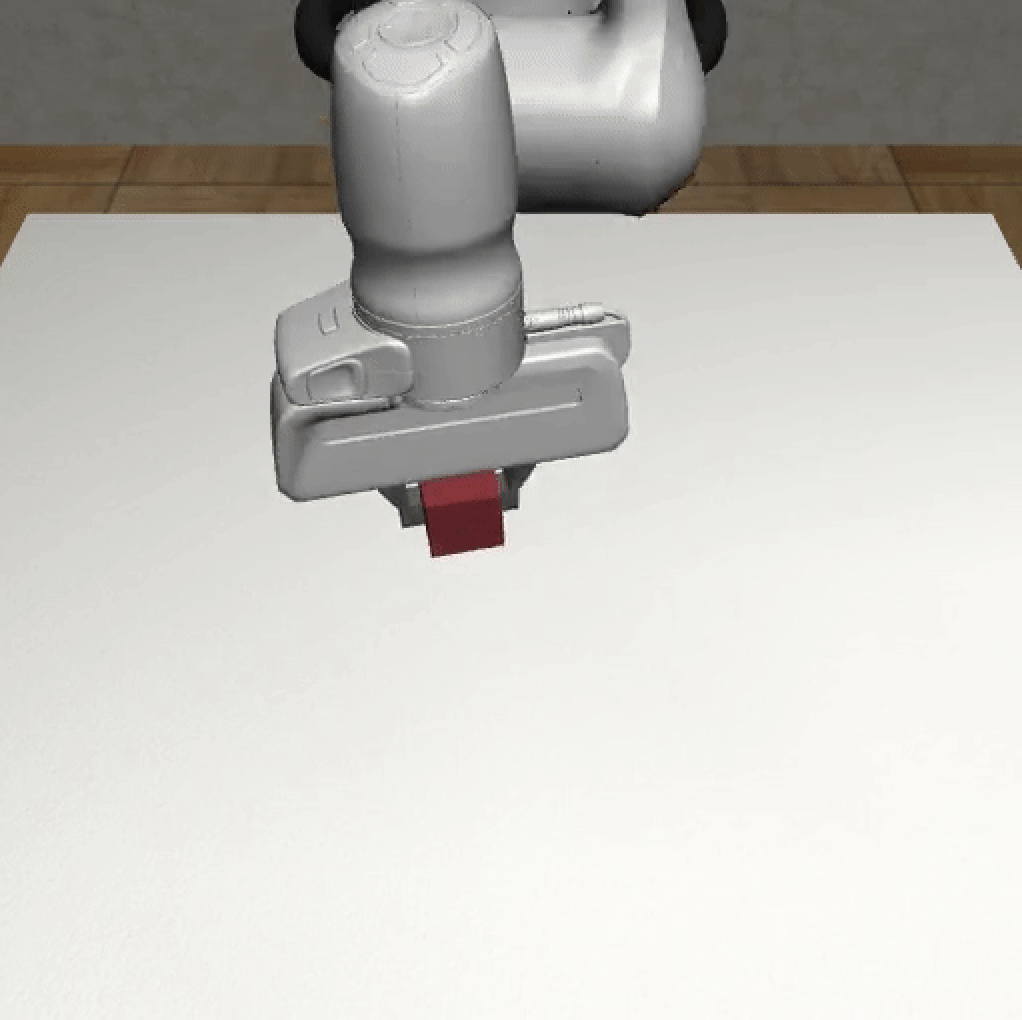
\includegraphics[width=.95\linewidth]{figs/task_lift.png}
    \centering
   \caption{The Lift task, where \\the goal is to pick a red cube \\off of the tabletop.}
  \label{fig:task_lift}
\end{minipage}%
    \centering
\begin{minipage}{.24\textwidth}

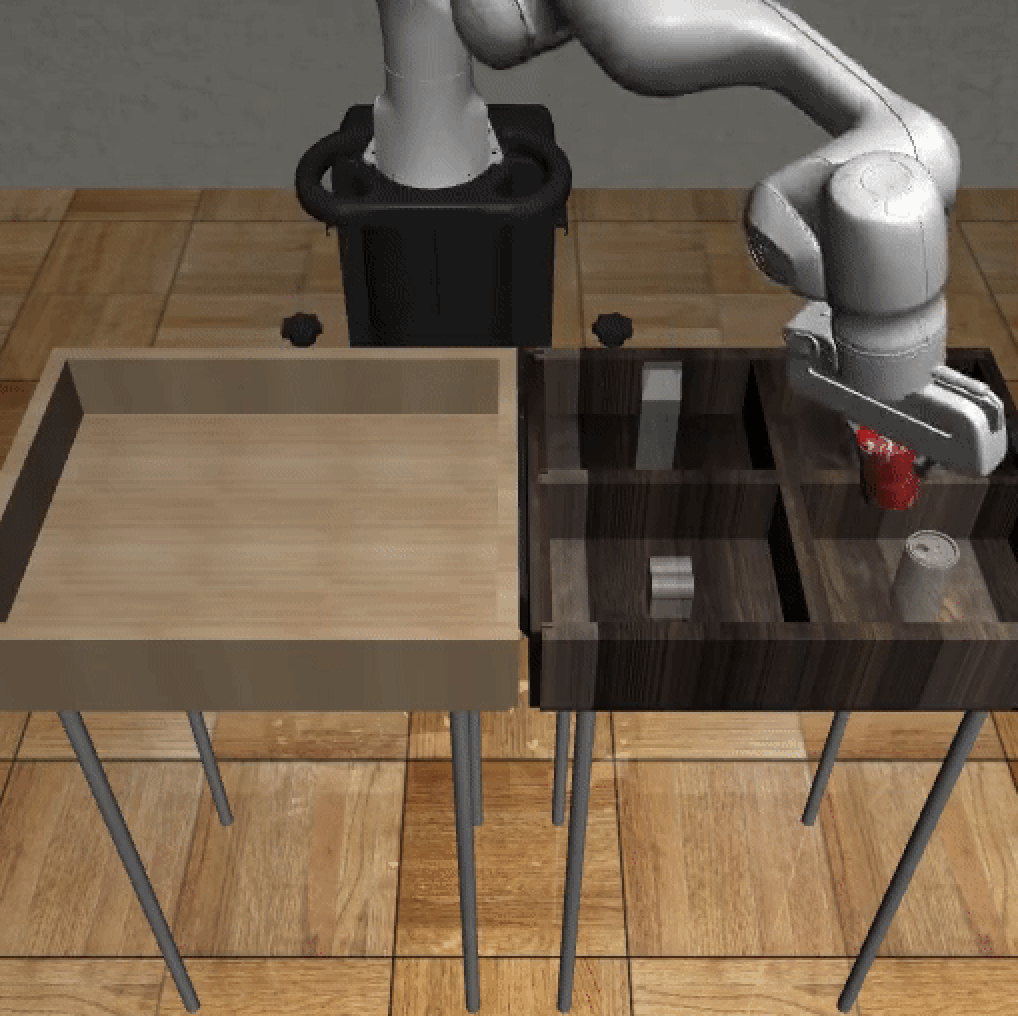
\includegraphics[width=.95\linewidth]{figs/task_can.png}
  \centering
  \caption{The Can task, where the goal is to pick up the red can and deposit it in the proper container.}
  \label{fig:task_can}
\end{minipage}
\end{figure}



\subsection{Semi-Sparse Reward Function}
The offline datasets in the original robomimic study use a binary reward function where the agent receives a reward of $1$ for successful completion of the task and $0$ at all other timesteps. Decision Transformer uses dense reward functions to differentiate between many different modes of policy quality \cite{decisiontransformer}. Therefore, our first step was to assign a more dense reward signal to robomimic's manipulation tasks. The robomimic codebase does provide an option to relabel datasets with robosuite's dense reward function. However, we found that the resulting rewards were not correlated with the quality of the dataset. In the Lift task dataset, for example, the proficient-human demos had the highest success rate but the lowest return values, while machine-generated data had the lowest success rate but the highest returns. This was a result of the worse quality demonstrations compensating for their low reward per timestep by taking much longer to solve the task, leading to a higher total return. To address the issue, we manually changed the reward function to include a semi-sparse success bonus. We added a large positive reward upon completion of the task which decreases with every timestep. Let $r_t^{\text{robomimic}}$ be the original dense reward term provided by the robomimic dataset at time $t$, and $d_t$ be a binary ``done" flag where $d_t = 1$ indicates successful task completion. We define a new reward term $r_t^{\text{DT}}$:
\vspace{-2.5mm}
\begin{align}
    r_t^{\text{DT}} = r_t^{\text{robomimic}} + d_t \max(500 - t, 0) 
    \label{eq:rt}
\end{align}

The success bonus decreases to zero after $500$ timesteps, which is the maximum length of the robomimic tasks. We relabel the offline dataset using Equation \ref{eq:rt}, and modify the reward function in the environment simulator for evaluation. This design lets our DT learn from a wide range of target values and improve its understanding of the quality of the sequence data, even in the presence of low-quality data.

\subsection{Decision Transformer Architecture}

% 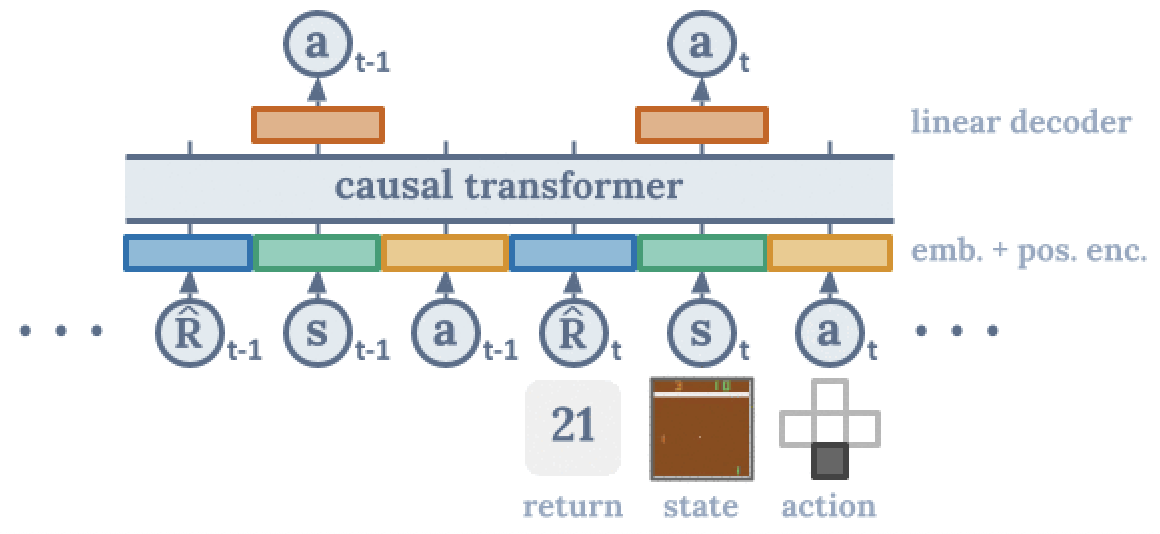
\includegraphics[width=0.5\textwidth]{figs/original.png}

 \noindent Our implementation is a modification of the original Decision Transformer architecture. The input format is a \textit{context sequence} of up to $k$ \textit{tokens}, where $k$ is the context length. Each token is a vector that concatenates a state $s_t$, return-to-go $\hat{R}_t$, and the previous action $a_{t-1}$\footnote{The first timestep of every trajectory is missing a previous action ($a_{-1}$), which we define as a zero vector.}. All sequences are padded to a length of $k$. The resulting sequence is projected to the embedding dimension of the Transformer architecture with a two-layer feedforward network. Transformers are permutation-invariant and require a position encoding to interpret the order of input tokens. The original Transformer \cite{transformer} used a hardcoded sinusoidal embedding. Instead, we randomly initialize embedding vectors for each of the $k$ position indices and train them alongside the rest of the model. This solution is more popular in domains with continuous inputs such as Vision Transformers \cite{dosovitskiy2020image}. The ($s, a, \hat{R}$) and position embeddings are summed together and form the input sequence of the core Transformer architecture. Our input format is a slight departure from the original DT, which embedded states, actions, and RTGs as separate consecutive tokens. Our concatenated version simplifies the implementation and position embedding while saving compute by reducing the overall sequence length by a factor of $3$.
 
 % This allows us to reduce the length of the sequences and the overall computational requirements of the model, as we only need to store a single token for each state-action pair instead of separate values for the state-action and return in the original decision transformer architecture.
 
 The embedded sequence of tokens is then fed into a causal Transformer, which uses a self-attention mechanism to model the dependencies between the tokens. We use a Pre-Norm Transformer \cite{xiong2020layer} architecture, which shifts the location of the layer normalization component to the residual branch. This is thought to improve stability early in training and enable deeper networks. The output of the Transformer is a sequence with the same dimensions as the embedded input. After a final normalization layer, this sequence is projected by a two-layer feedforward network into the dimension of the action distribution. The original DT uses a deterministic policy that outputs the action vector directly and is trained with mean squared error. We are focused on manipulation tasks with highly multi-modal demonstrations that would be difficult to model with a deterministic policy. Instead, our network generates the parameters of a stochastic distribution over actions. We implement a Gaussian policy with independent parameters for each dimension of the action space - a common default in the RL literature (e.g., \cite{schulman2017proximal, haarnoja2018soft}). We also add a Gaussian Mixture Model (GMM) policy based on robomimic that adds extra parameters in order to better represent multi-modal action distributions. We use the GMM parameterization with $5$ modes by default, and compare the two policy types in the Section \ref{sec:experiments}. A high-level summary of our DT model is depicted in Figure \ref{fig:arch}.
 
 
 % By using a multi-modal stochastic policy, our approach is able to capture the uncertainty and variability of continuous actions, resulting in improved performance compared to the deterministic policy used in the original paper \cite{decisiontransformer}.

% It is important to note that the original decision transformer uses a deterministic policy, where the action taken at each time step is determined by the current state and the previous actions with no uncertainty. In contrast, we train a multi-modal stochastic policy, where the action taken at each time step is modeled as a probability distribution over a range of possible actions. This allows us to better model continuous actions, where the exact action taken may vary within a certain range: 

% \begin{align}
% \pi(a|s) = P(A = a | S = s)
% \end{align}


% By using a multi-modal stochastic policy, our approach is able to capture the uncertainty and variability of continuous actions, resulting in improved performance compared to the deterministic policy used in the original paper \cite{decisiontransformer}. See Figure \ref{fig:arch} for more details.  \\

\begin{figure}[h!]
    \centering
    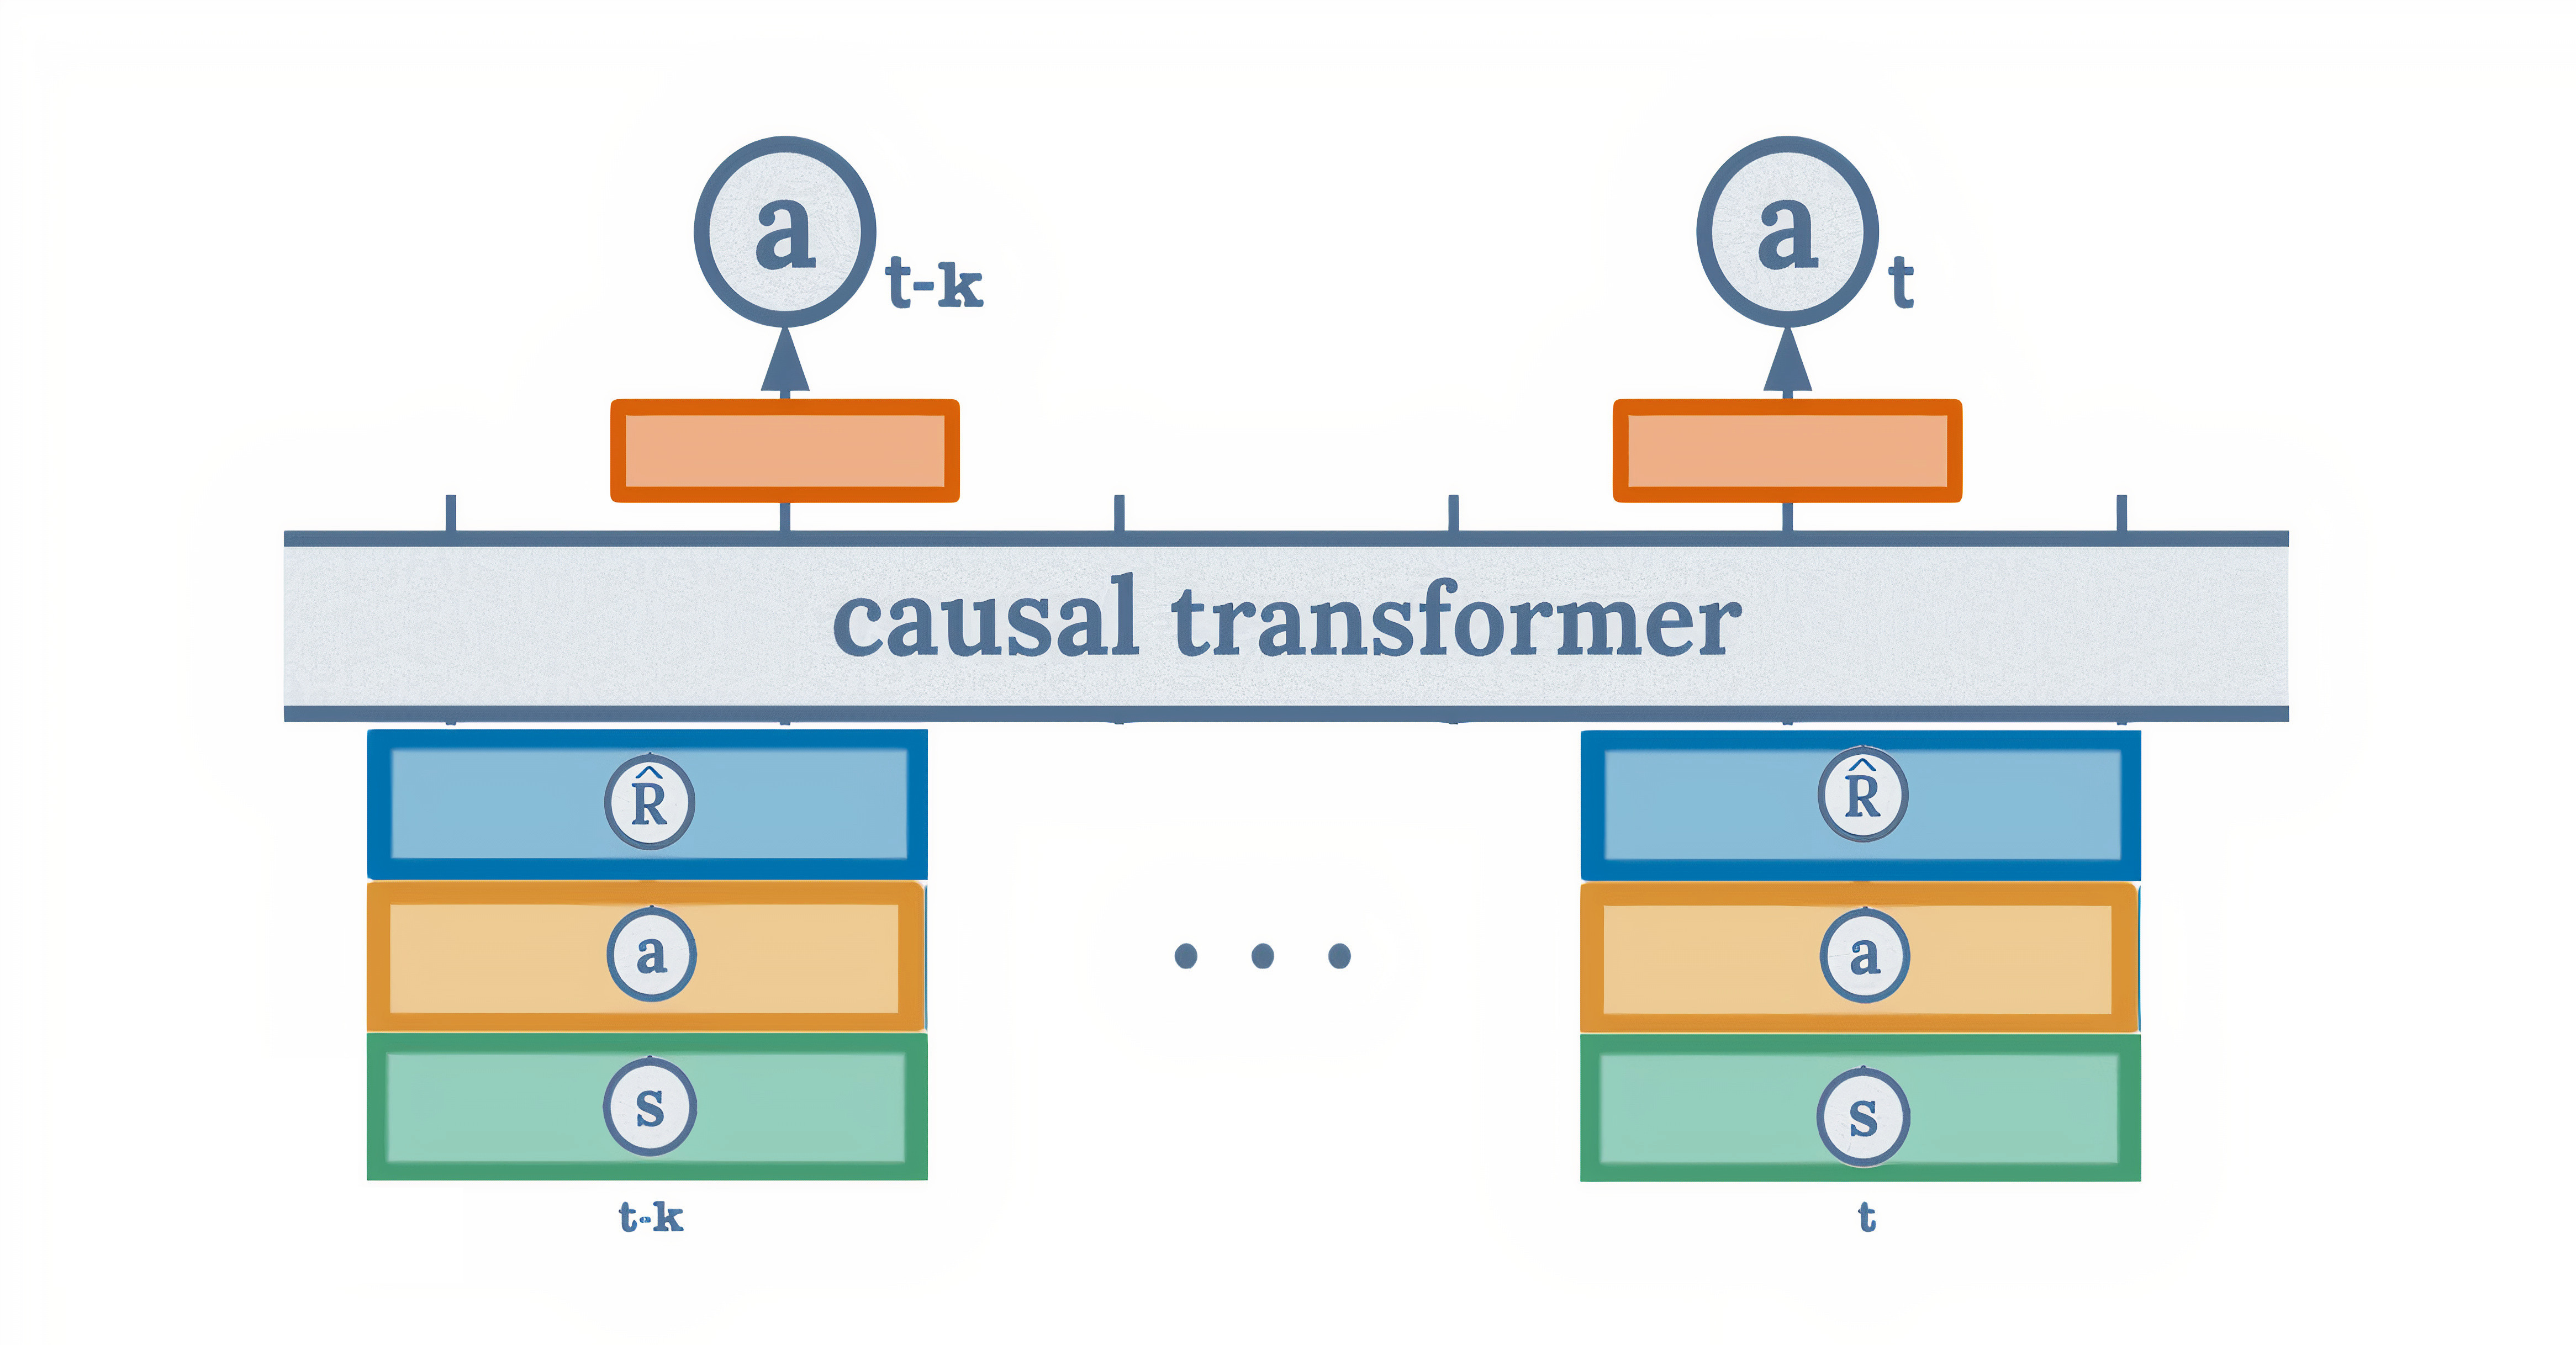
\includegraphics[width=.45\textwidth]{figs/arch.jpg}
    \caption{Our Decision Transformer architecture, with states, actions, and return-to-go values concatenated into one token. DT maps a context sequence of $k$ tokens to a sequence of $k$ action distributions.}
    \label{fig:arch}
\end{figure}


\subsection{Training}
Decision Transformer uses a standard sequence modeling objective and training loop. This can greatly simplify its implementation relative to many techniques in offline RL, where best practices are an open research topic \cite{kumar2021workflow}. We optimize our network parameters $\theta$ to maximize the probability of true actions in the dataset ($\mathcal{D}$) given the sequence of $k$ previous states, actions, and RTG values:

\vspace{-5mm}
\begin{align}
    c_t &:= (s_t, a_{t-1}, \hat{R}_t) \nonumber \\
    \theta^{\ast} &:= \mathop{\mathbb{E}}_{a_t, c_{t}, \dots, c_{t-k} \sim \mathcal{D}}[-\text{log}\pi_{\theta}(a_t \mid c_{t}, \dots, c_{t-k})]
    %\theta^{\ast} &:= \mathop{\text{argmin}}_{\theta}  \mathop{\mathbb{E}}_{a_t, c_{t-1}, \dots, c_{t-k} \sim \mathcal{D}}[-\text{log}\pi_{\theta}(a_t \mid c_{t-1}, \dots, c_{t-k})]
    \label{eq:loss}
\end{align}

We use several empirical best practices from the wider Transformer literature to stabilize training, including the AdamW optimizer \cite{loshchilov2017decoupled} and a linear learning rate warm-up for the first two thousand gradient steps \cite{transformer}. The batch size is fixed at $256$. Training is performed on a single NVIDIA GeForce RTX-3090 and takes roughly $6$ hours depending on model size. Much of the training time is consumed by evaluation rollouts in the simulated environments which are comparatively slow. We perform the evaluation in parallel across $8$ independent environments, batching and padding the sequences into one forward pass of the Transformer.
